\section{Appendix for multimodal and interdisciplinary composition}

\subsection{Further details on integrative ability results}
\begin{figure}[H]
\begin{AIbox}{\DV\ (some lines are merged for space saving)}
\begin{minted}[breaklines, breaksymbol=, baselinestretch=1, fontsize=\tiny]{html}
<HTML>
<head>
<style> canvas { border: 1px solid black; } button { margin: 10px; } </style>
<script>
  function randomInt(min, max) { // A function to generate a random integer between min and max (inclusive)
    return Math.floor(Math.random() * (max - min + 1) + min);
  }

  function randomColor() { // A function to generate a random color in hexadecimal format
    let hex = '#'; let chars = '0123456789abcdef';
    for (let i = 0; i < 6; i++) {
      hex += chars[randomInt(0, 15)];
    }
    return hex;
  }

  // A function to generate a random shape (circle, rectangle, triangle, or line) and draw it on the canvas
  function randomShape(ctx, width, height) {
    let shape = randomInt(1, 4); // 1 = circle, 2 = rectangle, 3 = triangle, 4 = line
    let x, y, r, w, h, x1, y1, x2, y2, x3, y3;
    let color = randomColor();
    ctx.fillStyle = color; ctx.strokeStyle = color; ctx.lineWidth = randomInt(1, 5);
    switch (shape) {
      case 1: // circle
        x = randomInt(0, width); y = randomInt(0, height); r = randomInt(10, 50);
        ctx.beginPath();
        ctx.arc(x, y, r, 0, Math.PI * 2);
        ctx.fill();
        break;
      case 2: // rectangle
        x = randomInt(0, width - 50); y = randomInt(0, height - 50); w = randomInt(10, 50); h = randomInt(10, 50);
        ctx.fillRect(x, y, w, h);
        break;
      case 3: // triangle
        x1 = randomInt(0, width); y1 = randomInt(0, height);
        x2 = randomInt(0, width); y2 = randomInt(0, height);
        x3 = randomInt(0, width); y3 = randomInt(0, height);
        ctx.beginPath();
        ctx.moveTo(x1, y1); ctx.lineTo(x2, y2); ctx.lineTo(x3, y3);
        ctx.closePath();
        ctx.fill();
        break;
      case 4: // line
        x1 = randomInt(0, width); y1 = randomInt(0, height);
        x2 = randomInt(0, width); y2 = randomInt(0, height);
        ctx.beginPath();
        ctx.moveTo(x1, y1); ctx.lineTo(x2, y2);
        ctx.stroke();
        break;
    }
  }

  // A function to generate a random Kandinsky painting on the canvas
  function generateKandinsky() {
    let canvas = document.getElementById('canvas');
    let ctx = canvas.getContext('2d');
    let width = canvas.width; let height = canvas.height;
    ctx.clearRect(0, 0, width, height); // Clear the canvas
    let bgColor = randomColor(); // Choose a random background color
    ctx.fillStyle = bgColor;
    ctx.fillRect(0, 0, width, height);
    let numShapes = randomInt(10, 20); // Choose a random number of shapes to draw
    // Draw each shape
    for (let i = 0; i < numShapes; i++) {
      randomShape(ctx, width, height);
    }
  }
</script>
</head>
<body>
  <h1>Random Kandinsky Painting Generator</h1>
  <button onclick="generateKandinsky()">Generate Kandinsky Painting</button>
  <canvas id="canvas" width="500" height="500"></canvas>
</body>
</html>
\end{minted}
\end{AIbox}
	\caption{Python code generated with the prompt ``Produce javascript code which generates random images in the style of the painter Kandinsky"}
	\label{fig:artprog1}
\end{figure}


\begin{figure}[H]
\begin{AIbox}{ChatGPT}
\begin{minted}[breaklines, breaksymbol=, baselinestretch=1, fontsize=\tiny]{html}
<!DOCTYPE html>
<html>
<head>
  <title>Kandinsky Generator</title>
</head>
<body>
  <button id="generate-button">Generate Kandinsky Painting</button>
  <canvas id="kandinsky"></canvas>
  <script>
    const canvas = document.getElementById('kandinsky');
    const ctx = canvas.getContext('2d');

    function generateKandinsky() {
      // Set the canvas size to a random value between 500 and 800 pixels
      canvas.width = Math.floor(Math.random() * 300 + 500);
      canvas.height = Math.floor(Math.random() * 300 + 500);

      // Set the background color to a random pastel color
      ctx.fillStyle = `hsl(${Math.random() * 360}, 50%
      ctx.fillRect(0, 0, canvas.width, canvas.height);

      // Draw a random number of circles with random sizes, positions, and colors
      const numCircles = Math.floor(Math.random() * 20 + 10);
      for (let i = 0; i < numCircles; i++) {
        const x = Math.random() * canvas.width;
        const y = Math.random() * canvas.height;
        const radius = Math.random() * 100 + 50;
        ctx.beginPath();
        ctx.arc(x, y, radius, 0, 2 * Math.PI);
        ctx.fillStyle = `hsl(${Math.random() * 360}, 50%
        ctx.fill();
      }
    }

    // Add an event listener to the button to generate a new Kandinsky painting when clicked
    const button = document.getElementById('generate-button');
    button.addEventListener('click', generateKandinsky);

    // Generate an initial Kandinsky painting
    generateKandinsky();
  </script>
</body>
</html>
\end{minted}
\end{AIbox}
	\caption{Python code generated with the prompt ``Produce javascript code which generates random images in the style of the painter Kandinsky"}
	\label{fig:artprog2}
\end{figure}

\begin{figure}[H]
\begin{AIbox}{\DV\ vs ChatGPT}
{\bf \DV:}\begin{minted}[breaklines, breaksymbol=, baselinestretch=1, fontsize=\tiny]{python}
# Define a function that calculates the body mass index (BMI) from weight and height
def bmi(weight, height):
    return weight / (height / 100) ** 2

# Define a function that checks if the blood test results are abnormal
def abnormal_results(results):
    # Assume the results vector has four elements: fasting glucose, HbA1c, triglycerides and HDL cholesterol
    # Define the normal ranges for each test according to the American Diabetes Association criteria
    normal_glucose = (5.6, 7.0) # mmol/L
    normal_hba1c = (5.7, 6.4) # %
    normal_triglycerides = (0.45, 1.7) # mmol/L
    normal_hdl = (1.0, 1.6) # mmol/L for men, (1.3, 2.2) for women
    
    # Check if any of the results are outside the normal ranges
    abnormal_glucose = results[0] < normal_glucose[0] or results[0] > normal_glucose[1]
    abnormal_hba1c = results[1] < normal_hba1c[0] or results[1] > normal_hba1c[1]
    abnormal_triglycerides = results[2] < normal_triglycerides[0] or results[2] > normal_triglycerides[1]
    if results[3] < normal_hdl[0] or (sex == "male" and results[3] > normal_hdl[1]) or (sex == "female" and results[3] > normal_hdl[3]):
        abnormal_hdl = True
    else:
        abnormal_hdl = False
    # Return True if any of the results are abnormal, False otherwise
    return abnormal_glucose or abnormal_hba1c or abnormal_triglycerides or abnormal_hdl

# Define a function that indicates if the patient is in increased risk for diabetes
def diabetes_risk(age, sex, weight, height, results):
    # Calculate the BMI from weight and height
    bmi_value = bmi(weight, height)
    # Define the BMI thresholds for overweight and obesity according to the World Health Organization criteria
    overweight = 25
    obesity = 30
    # Check if the patient is overweight or obese
    if bmi_value >= obesity:
        weight_status = "obese"
    elif bmi_value >= overweight:
        weight_status = "overweight"
    else:
        weight_status = "normal"
    
    # Check if the patient has abnormal blood test results
    abnormal = abnormal_results(results)
    # Define the age threshold for increased risk according to the American Diabetes Association criteria
    age_threshold = 45
    
    # Check if the patient is older than the age threshold
    old = age > age_threshold
    
    # Print a message indicating the patient's risk level based on the combination of factors
    if weight_status == "obese" and abnormal and old:
        print("You are in very high risk for diabetes. Please consult your doctor as soon as possible.")
    elif (weight_status == "obese" and (abnormal or old)) or (weight_status == "overweight" and abnormal and old):
        print("You are in high risk for diabetes. Please consult your doctor for further evaluation and advice.")
    elif (weight_status == "overweight" and (abnormal or old)) or (weight_status == "normal" and abnormal and old):
        print("You are in moderate risk for diabetes. Please monitor your blood sugar and cholesterol levels regularly and maintain a healthy lifestyle.")
    elif weight_status == "normal" and (abnormal or old):
        print("You are in low risk for diabetes. However, you may have some risk factors that need attention. Please check with your doctor if you have any symptoms or concerns.")
    else:
        print("You are in minimal risk for diabetes. Keep up the good work and stay healthy.")
\end{minted}
{\bf ChatGPT:}\begin{minted}[breaklines, breaksymbol=, baselinestretch=1, fontsize=\tiny]{python}
def is_at_risk(age, sex, weight, height, blood_tests):
    # Calculate body mass index (BMI)
    bmi = weight / (height ** 2)

    # Determine if the person is at increased risk based on age, sex, and BMI
    if (sex == "male" and age >= 45) or (sex == "female" and age >= 55):
        risk = True
    elif bmi >= 25:
        risk = True
    else:
        risk = False

    # Check blood test results to see if they indicate increased risk for diabetes
    for test in blood_tests:
        if test > normal_range:
            risk = True
            break

    return risk
\end{minted}
\end{AIbox}
	\caption{Python code generated with the prompt ``Produce python code for a program that takes as an input a patient's age, sex, weight, height and blood test results vector and indicates if the person is in increased risk for diabetes"}
	\label{fig:medprog}
\end{figure}







\subsection{Further details on vision results}\label{sec:visionappendix}

\begin{figure}
\begin{AIbox}{\DV}
Draw a photo using SVG inspired by the sentence

"A frog hops into a bank and asks the teller, 'Do you have any free lily pads?' The teller responds, 'No, but we do offer low interest loans for pond upgrades.'"

You are not allow to use extern images, textures but only basic shapes.
\tcbline
Can you add more details?
\tcbline
Add a roof to the bank

Make sure all the text on the top layer, it is covered by some object now.

Add 2 wheels to the car

Make the grass red

Add a woman on the right of the teller

Add a big red frog on the top left of the green frog.
\end{AIbox}
\caption{The prompts used to generate the 2D example in Section \ref{sec:2d3d_example}}\label{fig:2dprompt}
\end{figure}

\begin{figure}[H]
\begin{AIbox}{\DV}
Draw a 3D model in HTML using javascript and three.js inspired by the sentence "A fantasy landscape of floating islands, waterfalls, and bridges, with a dragon flying in the sky and a castle on the largest island."

The HTML file cannot use any external image or any texture, just plain colors.
\tcbline
The island arranges like the Olympic ring. Can you show how to edit the script such that the colors of the islands match the colors of the Olympic ring?
\tcbline
Hi, the color is correct but mislocated. Can you make sure each color is located as the Olympic rings lying horizontally?
\tcbline
The bridge arrangement is a bit off. Can you redesign which islands are connected to which island?
\tcbline
Can you add a few more dragons with different colors on different heights with different trajectories?
\tcbline
Somehow, I can only see 1 dragon in the code above.
\tcbline
Please make each dragon only use 1 color.
\tcbline
Put an island next to green island, opposite of the yellow island.

This island is special because it is not created by "createIsland".

This island looks like the End Island in Minecraft with the End City on the top.
\end{AIbox}
\caption{The prompts used to generate the 3D example in Section \ref{sec:2d3d_example}}\label{fig:3dprompt}
\end{figure}


\begin{figure}[H]
\begin{AIbox}{ChatGPT}
\parbox[t]{0.75\textwidth}{Produce TikZ code that draws a person composed from letters in the alphabet. The arms and torso can be the letter Y, the face can be the letter O (add some facial features)  and the legs can be the legs of the letter H. Feel free to add other features.}\hspace{50px}
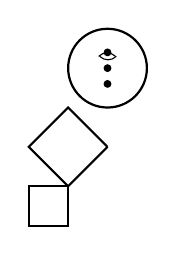
\begin{tikzpicture}[scale=0.5,baseline={(0,0.8)}]

\draw[thick] (0,0) -- (-1,1) -- (-2,0) -- (-1,-1) -- (0,0);

\draw[thick] (0,2) circle (1);
\draw (0.2,2.3) arc (45:135:0.3);
\draw (-0.2,2.3) arc (225:315:0.3);

\draw[thick] (-1,-1) -- (-1,-2) -- (-2,-2) -- (-2,-1) -- (-1,-1);

\fill[black] (0,2.4) circle (0.1);
\fill[black] (0,2) circle (0.1);
\fill[black] (0,1.6) circle (0.1);

\end{tikzpicture}
\tcbline
\parbox[t]{0.75\textwidth}{Please add a shirt and pants.}\hspace{50px}
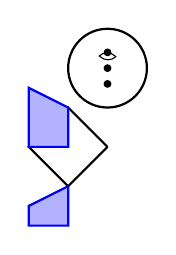
\begin{tikzpicture}[scale=0.5,baseline={(0,0.3)}]

\draw[thick] (0,0) -- (-1,1) -- (-2,0) -- (-1,-1) -- (0,0);

\draw[thick, blue, fill=blue!30] (-1,1) -- (-2,1.5) -- (-2,0) -- (-1,0) -- (-1,1);

\draw[thick, blue, fill=blue!30] (-1,-1) -- (-2,-1.5) -- (-2,-2) -- (-1,-2) -- (-1,-1);

\draw[thick] (0,2) circle (1);
\draw (0.2,2.3) arc (45:135:0.3);
\draw (-0.2,2.3) arc (225:315:0.3);

\fill[black] (0,2.4) circle (0.1);
\fill[black] (0,2) circle (0.1);
\fill[black] (0,1.6) circle (0.1);

\end{tikzpicture}

\end{AIbox}

\begin{AIbox}{ChatGPT}\scriptsize\vspace{-5px}
\parbox{1\textwidth}{\begin{alltt}
You will be given a name of an object (such as Car, Chair, Elephant) and a letter in the alphabet. Your goal is to first produce a 1-line description of how that object can be combined with the letter in an image (for example, for an elephant and the letter J, the trunk of the elephant can have a J shape, and for the letter A and a house, the house can have an A shape with the upper triangle of the A being the roof). Following the short description, please create SVG code to produce this (in the SVG use shapes like ellipses, triangles etc and polygons but try to defer from using quadratic curves).\\

Round 1: A pig and the letter H. \\
\hl{The pig's tail can be shaped like the letter H.}

Round 2: A house and the letter U. \\
\hl{The house's roof can be shaped like the letter U.}

Round 3: A chair and the letter K. \\
\hl{The backrest of the chair can be shaped like the letter K.}

Round 4: A dog and the letter Q. \\
\hl{The dog's tail can be shaped like the letter Q.}

Round 5: A car and the letter E. \\
\hl{The car's front grill can be shaped like the letter E.}
\end{alltt}
}
\begin{center}
\includegraphics[width=0.7\textwidth]{Section 2/letters_objects2.png}
\end{center}
\end{AIbox}
	\caption{A stick figure composed of alphabet symbols and Images combining alphabet letters and objects.}
	\label{fig:visionchatgpt}
\end{figure}
\begin{figure}[h]
	\centering
	\includegraphics[height=0.16\textwidth]{Section 2/cifar2.png}
	\caption{SVGs generated by ChatGPT \ for the classes automobile, truck, cat, dog.}
	\label{fig:2dchat}
\end{figure}
\subsection{Graphic novel design example}
\begin{AIbox}{\DV}\scriptsize\vspace{-5px}
\parbox{1\textwidth}{\begin{alltt}
I'd like to write a one page graphic novel for little girls, do you have any idea of what I could do? \\

\lightgreen{ Possible one page graphic novels for little girls:

- A girl who loves to draw discovers a magic crayon that brings her creations to life, and uses it to make friends with a unicorn, a dragon, and a fairy.

- A girl who dreams of becoming a detective solves a mystery at her school, finding clues, suspects, and a hidden treasure in the library, the cafeteria, and the playground.

- A girl who is afraid of the dark learns to overcome her fear with the help of a friendly star, who guides her through a nighttime adventure full of wonders and surprises.

- A girl who loves to bake enters a contest to create the most delicious and original cupcake, and faces challenges, rivals, and judges along the way, but also finds support and inspiration from her family and friends.

- A girl who wants to play soccer with the boys proves her skills and courage by joining a secret league of girls who play at night, wearing masks and capes, and using special moves and gadgets. } \\

I love the first idea, let's make it even simpler, just a girl who loves to draw and discovers a magic crayon that she uses to bring a unicorn to life. Can you help me realizing that one page graphic novel? \\

\lightgreen{ Possible steps to realize that one page graphic novel:

- Sketch out a rough layout of the page, dividing it into panels of different sizes and shapes according to the flow of the story. For example, you could use a large panel for the opening scene, where the girl is drawing in her room, then smaller panels for the moments when she finds the magic crayon, draws the unicorn, and sees it come to life, and then a final large panel for the ending scene, where she hugs the unicorn and smiles.

- Write the dialogue and captions for each panel, using simple and expressive language that matches the tone and mood of the story. For example, you could use a caption to introduce the girl and her hobby, then have her say things like "Wow, what a cool crayon!", "I wish I had a unicorn friend", and "You're real!" to show her curiosity, desire, and joy. You could also use sound effects to add some drama and humor, such as "Scribble, scribble", "Poof!", and "Neigh!"

- Draw the characters and backgrounds for each panel, using a clear and colorful style that appeals to little girls. For example, you could make the girl cute and expressive, with big eyes, long hair, and a dress, and the unicorn majestic and friendly, with a horn, a mane, and a tail. You could also add some details and accessories to make them more unique and interesting, such as a flower in the girl's hair, a star on the unicorn's forehead, or a poster of a fairy tale on the wall. 

- Ink and color the panels, using a pen, a brush, or a digital tool to outline and fill in the shapes and textures. For example, you could use black ink for the outlines, and bright colors for the characters and backgrounds, such as pink, purple, and blue. You could also use some shading, highlights, and patterns to create some depth and contrast, such as a gradient for the sky, a sparkle for the magic crayon, or a stripe for the unicorn's coat.

- Add the dialogue and captions, using a font, a lettering, or a handwriting that fits the style and voice of the story. For example, you could use a round and bubbly font for the girl's speech, and a script and elegant font for the captions, and place them in balloons and boxes that match the shape and size of the panels. You could also use some effects and variations to emphasize some words or emotions, such as a bold or italic font, a bigger or smaller size, or a different color or shape. } \\

That sounds really amazing. Can you write SVG code that produces this one page graphic novel? \\

\lightgreen{ [...] here is a possible example of SVG code [...]. [Output of SVG code below.] }
\end{alltt}
}
\begin{center}
	\includegraphics[width=0.5\textwidth]{figures/novel.png}
\end{center}
\end{AIbox}

